\documentclass[11pt]{article}
\usepackage[margin=1in]{geometry}
\usepackage[T1]{fontenc}
\usepackage{lmodern}
\usepackage{booktabs}
\usepackage{graphicx}
\usepackage{amsmath}

\title{GPU Device Information Report}
\author{Trinh Thanh Vinh}
\date{September 29, 2026}

\begin{document}

\maketitle

\section{Objective}

The purpose of this labwork was to use \texttt{numba.cuda} to select a CUDA device and display basic information about the GPU.

\section{Results}

The selected device was device 0. The information obtained from the program is summarized below.

\begin{center}
\begin{tabular}{ll}
\toprule
Property & Value \\
\midrule
Device ID & 0 \\
Device name & NVIDIA GeForce RTX 3060 \\
Multiprocessor count & 28 \\
Cores per multiprocessor & 128 \\
CUDA core count & 3584 \\
Compute capability & 8.6 \\
Total memory & 12.0 GiB (12,884,377,600 bytes) \\
Free memory at execution & 10.98 GiB (11,789,139,968 bytes) \\
\bottomrule
\end{tabular}
\end{center}

There is no built-in function in \texttt{numba.cuda} to directly retrieve the number of CUDA cores. However, the number of CUDA cores can be calculated using the formula:
\[
\text{CUDA cores} = \text{Multiprocessor count} \times \text{Cores per multiprocessor}
\]
\section{Captured Output}

Figure~\ref{fig:gpu-output} shows the output produced by the Python program.

\begin{figure}[ht]
    \centering
    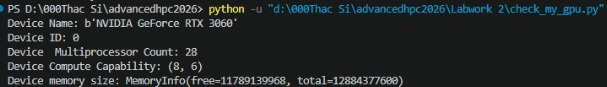
\includegraphics[width=\textwidth]{image.png}
    \caption{GPU information displayed by the \texttt{numba.cuda} program.}
    \label{fig:gpu-output}
\end{figure}


\section{Conclusion}

The \texttt{numba.cuda} library successfully detected and selected the NVIDIA GPU. It provided the device name, ID, multiprocessor count, compute capability, and memory information.

\end{document}